\chapter{Method}
\label{chap:method}

This chapter entails the details of the neural network such as the architecture, loss/objective function along with the training and evaluation procedures of the proposed method. Other choices such as activation functions, optimizers, initialization, etc that completes the architecture are presented later in chapter \ref{chap:experiments} Experiments, along with the reasoning behind the choices and the compilation of essential components required to reproduce the entire network.
% FIXME experiments and reproduction

\section{Architecture}
To predict root-relative 3D pose solely using 2D poses, a hybrid network using \ac{vae} and \ac{gan} as discussed in \ref{subsec:vaeganhybrid} is employed. In contrast to the \ac{vae}-\ac{gan} hybrid proposed by \cite{autoencoding_beyond_pixels}, the \ac{gan} loss gradient is propagated to both the decoder and the encoder. In other words, the \ac{vae} as a whole is considered as the generator network. The overall architecture is composed of 3 models Encoder, Decoder, and Discriminator as illustrated in Fig \ref{fig:method_arch}. This section elaborates on each of the models and how they are interconnected. 
%FIXME activation in the experiment

\subsection{Encoder}
Adding to the explanation of \ac{vae} in \ref{subsec:vae}, the role of the encoder $Q$, is to take a 2D pose $\textbf{x}_i = (x_i, y_i)$ with its root located at the joint and of upper body length of $c$ units as an input. Where $i = 1 ... J$ and $J$ denote the number of joints of the pose. And output the corresponding embedding in a $d$ dimensional latent space in the form of mean $\mu$ and standard deviation $\sigma$ of each dimension.

\begin{equation} \label{eqn:Q_fn}
    \begin{gathered}[b]
        Q_{\theta_q}(\textbf{x}) = \mu, \sigma
    \end{gathered}
\end{equation}

Where $\theta_q$ denotes the learned parameters of the encoder during training. This encoder is composed of an upsampling layer that scales the $2\!\cdot\!J$ dimensional input to match the number of hidden neurons $h$ of the encoding module. The encoding module $q$ is made of $n$ residual block composed of 2 \ac{fc} layers following the related works, to allow comparison. This residual block structure is repeated for the decoder and the discriminator. The encoding block is followed by 2 \ac{fc} (linear) layers that downsample the hidden representation of dimension $h$ to match the latent space dimension $d$. The output of the two downsampling layers represents the mean and standard deviation respectively. However, in practice, the encoder is designed to predict log-variance instead of the standard deviation to have a better distribution of values and gradient. The layers of the encoder, decoder, and the discriminator models are kept similar for simplicity and as done by the related works. The residual blocks used in all the 3 models are identical and is illustrated in Fig \ref{fig:residual_block}.

Both \ac{fc} layers of the residual block are followed by batch normalization, activation, and dropout layers of the same dimensionality. While other \ac{FC} layers are only followed by an activation function. The linear layers in the residual blocks of the \ac{vae} contain weights but do not have the bias component.


\begin{figure}[h] 
    \centering
    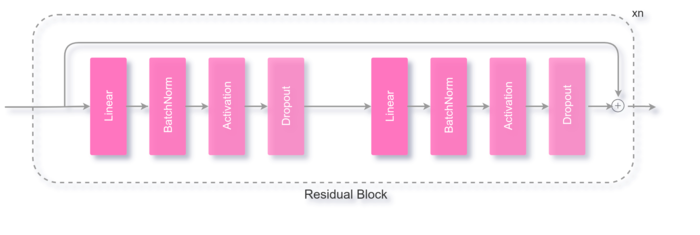
\includegraphics[width=\textwidth]{figures/arch/res_block.png}
    \caption{Illustration of the residual block made of 2 Linear layers of the same input and output dimensionality. The intermediate BatchNorm, activation, and dropout layers maintain the same dimensionality. These blocks are repeated $n$ times based on the configuration of the model.
    }
    \label{fig:residual_block}
\end{figure}

\subsection{Decoder}
The decoder $P$ takes the 2D pose embedding $z$ derived from the mean and log-variance predicted by the encoder and estimates the corresponding 3D pose $\textbf{Y}_i = (x^\prime_i, y^\prime_i, z^\prime_i)$. Similar to the encoder, $i = 1 ... J$ and $J$ denote the number of joints of the pose. The reparametrization trick is used to make the process differentiable and induce variance. This is done by scaling the standard deviation obtained from the log-variance with a random sample $\epsilon$ from a unit gaussian distribution $\mathcal{N}(0,1)$. The sum of the scaled standard deviation and the mean gives the sample $z$.

\begin{equation} \label{eqn:P_fn}
    \begin{gathered}[b]
        z = \mu + \sigma \odot \epsilon \\
        P_{\theta_p}(z) = \textbf{Y}
    \end{gathered}
\end{equation}

Where $\theta_p$ represents the learned parameters of the decoding network. Similar to the encoder, the decoder consists of an upsampling layer that scales the sample $z$ of dimensionality $d$ to match the number of hidden neurons $d$ in the decoding module. The decoding module is identical to the encoding module and consists of $n$ residual blocks similar to that of the encoder. This decoding module is followed by a \ac{fc} layer to downsample the neurons to predict the 3D pose of dimensions $3\!\cdot\!J$. As the goal is to predict root-relative pose with the root at the origin, the output joints are considered to be relative to the origin (0, 0, 0).

Since the predicted 3D pose is to be projected to back to the 2D pose to form the reconstruction loss, the distance between the head and the pelvis joint should approximately be of unit length as explained in \ref{sec:processing}. To achieve this, a Tanh activation function is used at the downsampling/output layer to obtain the predicted 3D pose (all joints) in the range [-1, 1].

\subsection{Reprojection}
\label{subsec:reproject}
Referring to the camera modeling section \ref{sec:camera_projection}, the 3D that corresponds to the pre-processed 2D pose is located at a fixed distance $c$ from the camera. The 3D pose is considered to be predicted relative to the origin for simplicity and symmetry and is to be translated $c$ units aways from the camera. Another required adjustment is the scale. The range of coordinates predicted is in the range [-1,1]. But the length of the lower half of the pose can be longer than the upper half and usually is the case. Hence the predicted 3D pose is scaled by a factor of 1.3, which is the ratio of the mean length of the upper and lower halves. This is to enforce that the length of the upper half is ~1 unit while covering the true range of the lower half and get the best 2D re-projection.

This scaled 3D pose prediction is directly projected from the same point of view to get a 2D projection that corresponds to the input 2D pose. This similarity is used as the reconstruction loss for constrained optimization of the \ac{vae}.

\begin{equation} \label{eqn:proj_direct}
    \begin{gathered}[b]
        \textbf{Y}^\prime = \textbf{Y}*1.3 + (0,0,c) \\
        \textbf{y} = PP(\textbf{Y}^\prime)
    \end{gathered}
\end{equation}

Where PP refers to perspective projection and \textbf{y} denotes the 2D projection that corresponds to the input 2D pose. The scaled 3D pose is also randomly rotated by uniformly sampling an azimuth angle from the range [$-\pi, \pi$] and elevation range in the range [$-\pi/9, \pi/9$]. The 2D pose obtained from the projection of this rotated 3D pose gives a different point of view, a \textbf{\textit{novel view}} of the 3D pose that is different from the views of the subject in the dataset. This novel view is used for unconstrained optimization of the \ac{vae} using the discriminator. The elevation angle has been followed by other works but is not observed to have any visible impact.

\begin{equation} \label{eqn:proj_rotated}
    \begin{gathered}[b]
        \textbf{Y}^\prime_{rot} = \textbf{R} * (\textbf{Y}*1.3) + (0,0,c) \\
        \tilde{\textbf{y}} = PP(\textbf{Y}^\prime_{rot})
    \end{gathered}
\end{equation}

Where \textbf{R} refers to the rotation matrix formed using the randomly sampled angles. $\tilde{\textbf{y}}$ refers to novel view of the 3D pose.

\subsection{Discriminator}
The discriminator takes the novel view 2D pose of the predicted 3D pose $\tilde{\textbf{y}}$ along with the real 2D poses \textbf{x} from the dataset as the input and classifies which 2D pose belongs to which category, real or fake (generated novel view). The real and novel views need not correspond to the same pose, the goal of the discriminator is to learn the general ability to distinguish the 2D poses from the dataset (real) from the predicted poses (fake).

\begin{equation} \label{eqn:proj_rotated}
    \begin{gathered}[b]
        D_{\theta_d}(\tilde{\textbf{y}} \cup \textbf{x}) = \left\lbrace p_{class}^i | i \in {1, .. n(\tilde{\textbf{y}} \cup \textbf{x})}\right\rbrace \\
        where, 0\leq p_{class} \leq 1
    \end{gathered}
\end{equation}

Where $\theta_d$ refers to the learned parameters of the discriminator and $p_{class}$ here denotes the probability of the pose's class, with 1 being real and 0 being fake. The discriminator mimicking the encoder and the decoder upsamples the $2\!\cdot\!J$ dimensional novel 2D pose to $h$ dimensions of the main module. The main module just as other models are composed of $n$ residual blocks. However, the batch normalization layer is removed in the discriminator's residual blocks following standard practices. It is important to note that $n$ need not be the same for all the 3 models. The learned features are downsampled to predict the probability of the pose being real or fake. The sigmoid activation function is used at this last layer as the required values are in the range [0, 1].

\begin{figure}[h] 
    \centering
    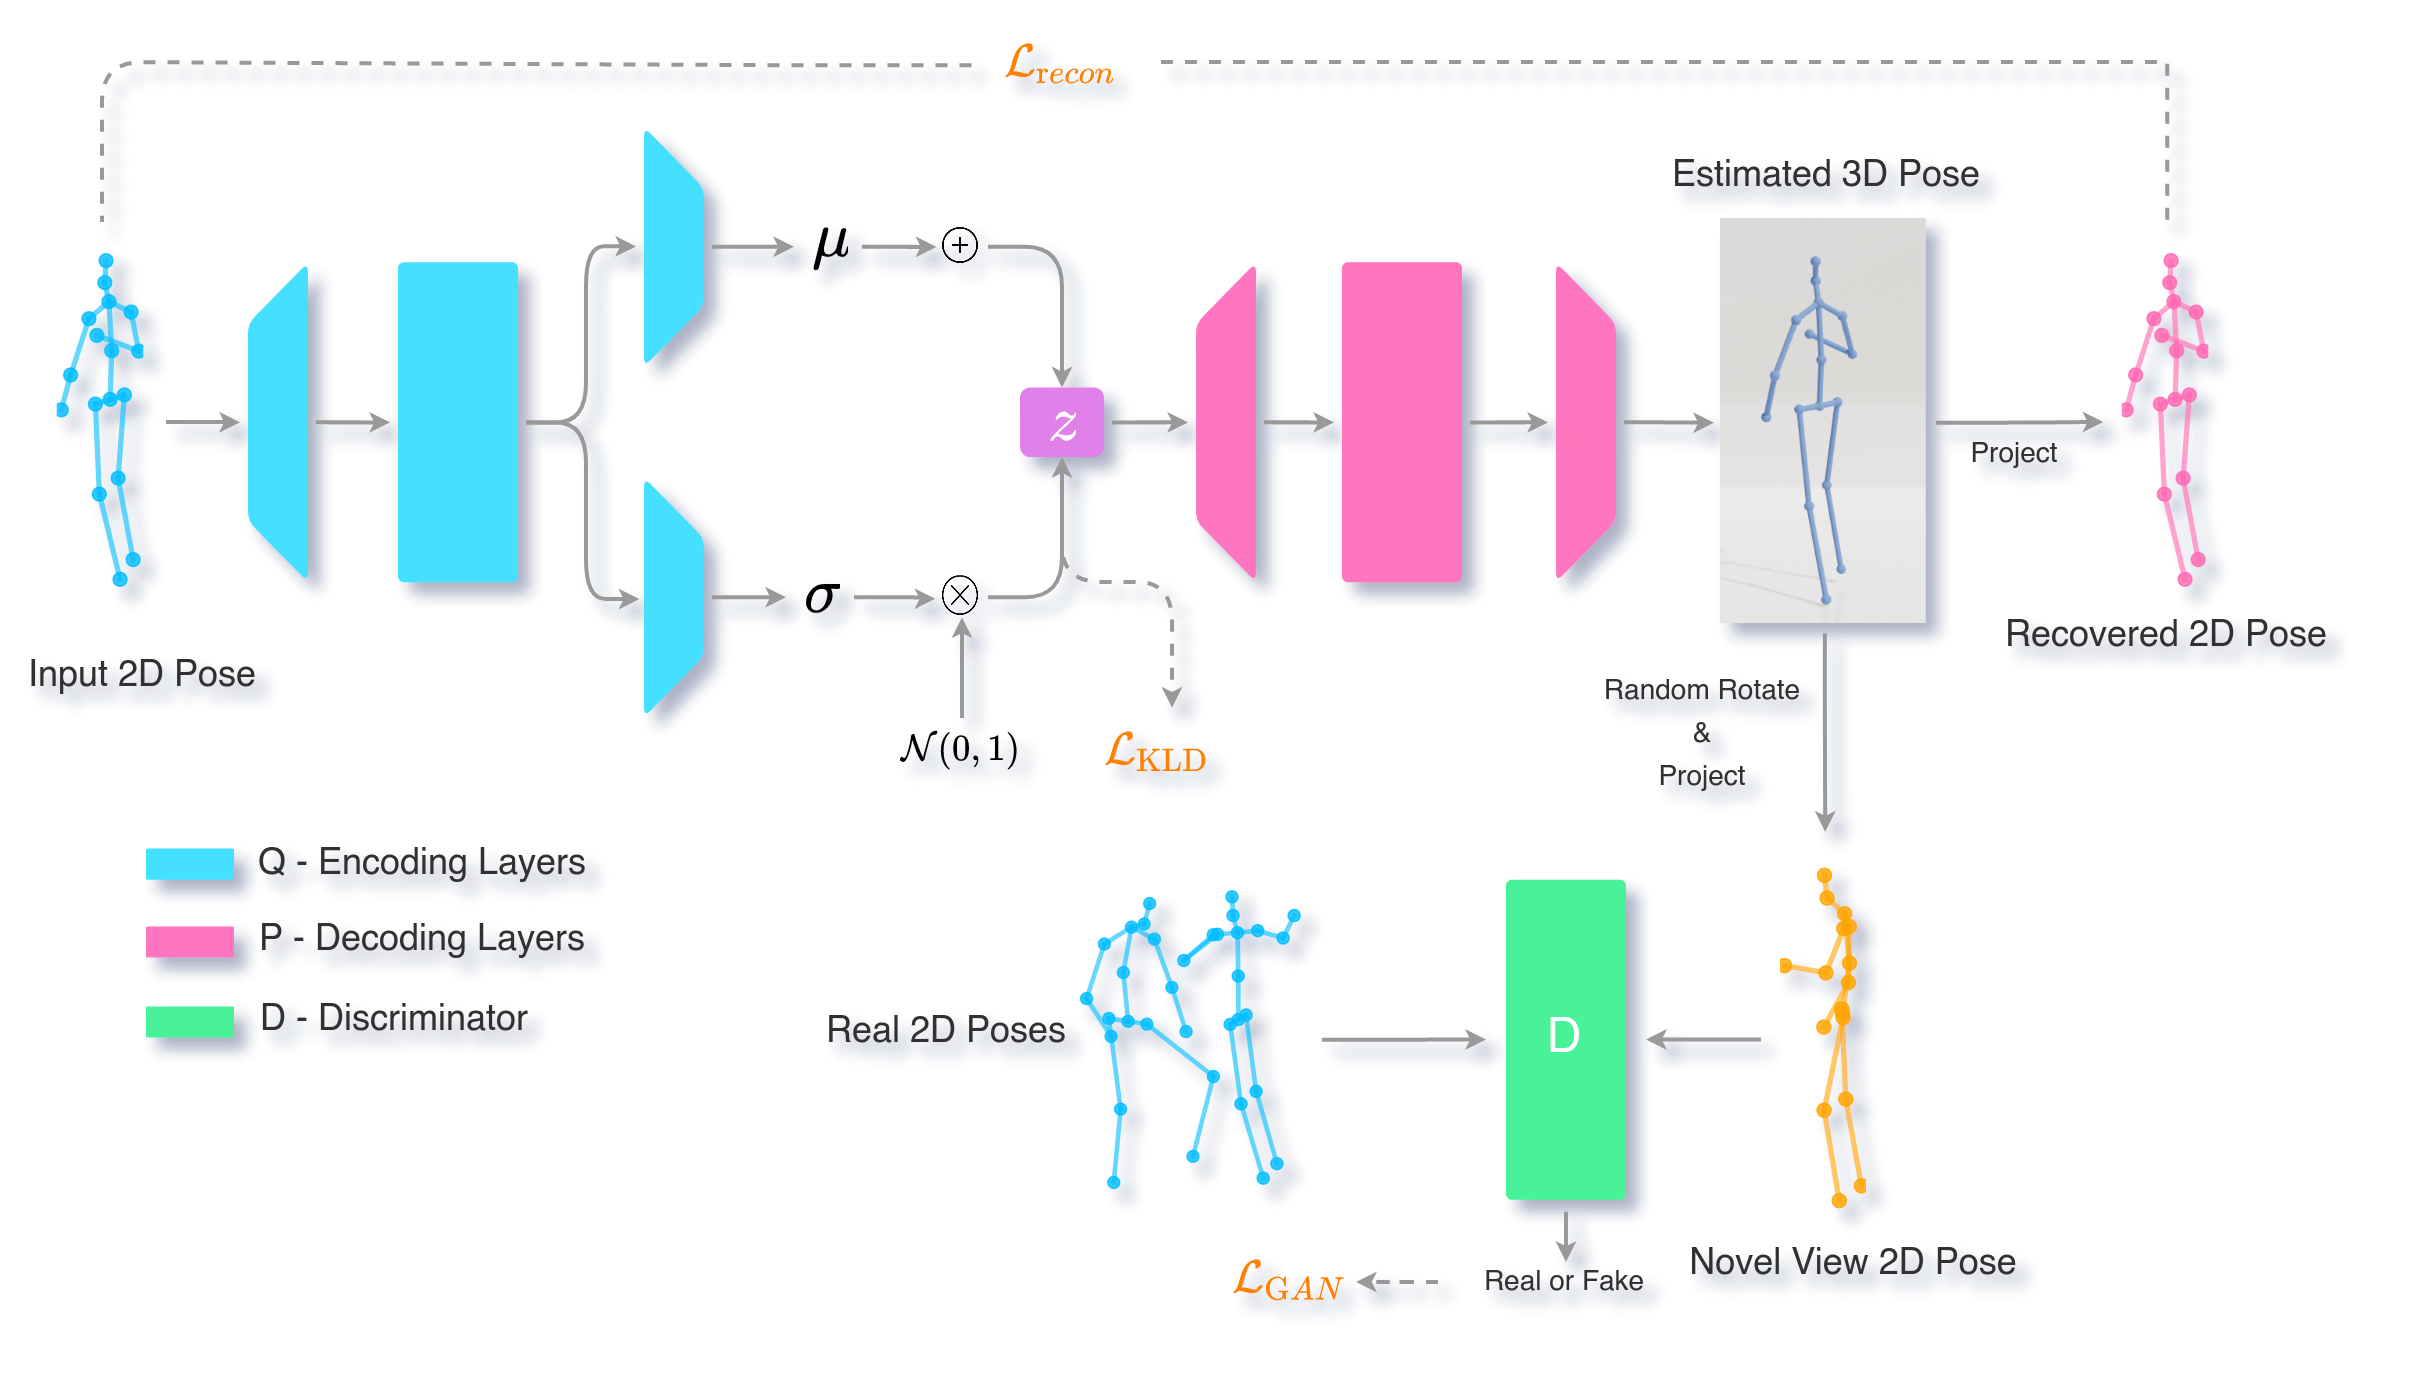
\includegraphics[width=\textwidth]{figures/arch/method_arch.png}
    \caption{Illustration of the neural architecture of the proposed method. The network components in blue, encode the 2D pose to a latent representation in terms of mean $\mu$ and standard deviation $\sigma$ of the distribution. While the components in pink, sample $z$ from this latent space and decode the corresponding 3D pose. The 3D pose is projected directly to 2D space for a constrained optimization using the input 2D pose in the camera view and randomly rotated and projected for unconstrained optimization using the discriminator $D$ in a novel angle. The data that contributes to the loss function in orange, is mapped with a dotted line.
    }
    \label{fig:method_arch}
\end{figure}

\section{Loss Functions}
\label{sec:loss_fn}
The loss functions used in this \ac{vae}-\ac{gan} are similar to the ones explained in \ref{subsec:vaeganhybrid}. The hybrid training proposed in \cite{autoencoding_beyond_pixels} uses the similarity between the prediction and input estimated by the discriminator \textit{replacing} the element-wise loss. While the proposed approach exploits the element-wise loss and the similarity loss by using them on different transformations of the prediction (direct view 2D and novel view 2D). The formulation of each loss function of the hybrid with respect to the human pose data is as follows.

\subsection{Reconstruction Loss}
Since the goal of the proposed method is to learn 3D pose without requiring any of such training data, the approach uses 2D pose as its supervisory data. This self-supervision is achieved by reprojecting the 3D pose in the same view to retrieve the 2D pose that should ideally be the same as the input 2D pose as discussed in the Reprojection \ref{subsec:reproject} part of the previous section. The objective of the model here is to converge the distance (element-wise) between the predicted 2D pose $\textbf{y}$ and the input 2D pose $\textbf{x}$. L1 loss is used to measure the element-wise reconstruction error.

\begin{equation} \label{eqn:loss_recon}
    \begin{split}
        \mathcal{L}_{\text {recon}}  & = L1\_loss(\textbf{x}, \textbf{y}) \\
        & = \sum_{i=1}^J |\textbf{x}_i - \textbf{y}_i|
    \end{split}
\end{equation}

The training of the hybrid network with 3 different losses is not very stable. For the reconstruction loss, there is an absolute target and metric for learning. So this is a constrained optimization and directly corresponds to the error of the 3D pose. Hence it is desired to give high priority and keep this loss relatively stable and low. All the 3 loss terms are weighted to be summed to one final object term that is used to update the network. The weight coefficient $\lambda_{recon}$ is kept constant and relatively higher than the other two that are introduced next.

\subsection{Latent Prior Loss}

The proposed hybrid though named \ac{vae}-\ac{gan}, actually uses a \ac{bvae}, it is not highlighted as the only difference is having a variable coefficient rather than fixing it to 1. Referring to the explanation of the \ac{bvae} in \ref{subsec:bvae}, the higher the weight of the \ac{kld} term the better is the disentanglement or clustering of the embeddings are in the latent space. There is no magic $\beta$ that gives the best reconstruction and representation. This is a trade-off and the value is chosen based on the requirements. Though both are the priorities of this work, more importance is given to the reconstruction as it is quantitative. It is important to note that the weight coefficient $\lambda_{KLD}$ to balance the loss terms are separated for the $\beta$ term to have better control when conducting experiments with different scheduling strategies for the $\beta$ term. A cyclic beta technique similar to \cite{cyclicbeta} is used to handle the vanishing \ac{kld} problem, where $\beta$ is increased from 0 to true value every $b$ epochs and observed to improve training.

\begin{equation} \label{eqn:loss_kld}
    \begin{split}
        \mathcal{L}_{\text {prior}} = \mathcal{L}_{\text {KLD}} &= -0.5 * \sum (1 + log(\sigma^2) - \mu^2 - \sigma^2) \\
        &= -0.5 * \sum (1 + logvar - \mu^2 - e^{logvar})
    \end{split}
\end{equation}

The $logvar$ term here is the output of one of the downsampling layers of the encoder in practice. The terms denoted in the equation are per sample and in practice, the losses are averaged and normalized based on the dimensionality. The normalization is included in their $\lambda$ coefficients.

\subsection{Discriminator Loss}

The discriminator takes both the samples from the real dataset \textbf{x} and predicted novel 2D poses $\tilde{\textbf{y}}$ and classifies the samples. For making such training data the values of 1s and 0s are given as the labels for the real and generated 2D poses respectively. As the labels are self-generated the discriminator training is self-supervised as well. In contrast to the reconstruction error, the error in discriminator's classification is not expected to be minimized even though the models are learning to minimize this metric. Rather, the role it plays is to help the generator produce 3D poses that give more realistic 2D novel views. That is 2D projections from random views of the 3D pose that are indistinguishable from the 2D pose from the real dataset. Fig \ref{fig:novel_view_constraint} illustrates the differences in the novel views of realistic and unrealistic 3D poses that this adversarial training aims to resolve. Hence this error is used to optimize both the discriminator and generator models that produce the 3D poses.

\begin{figure}[h]
    \centering
    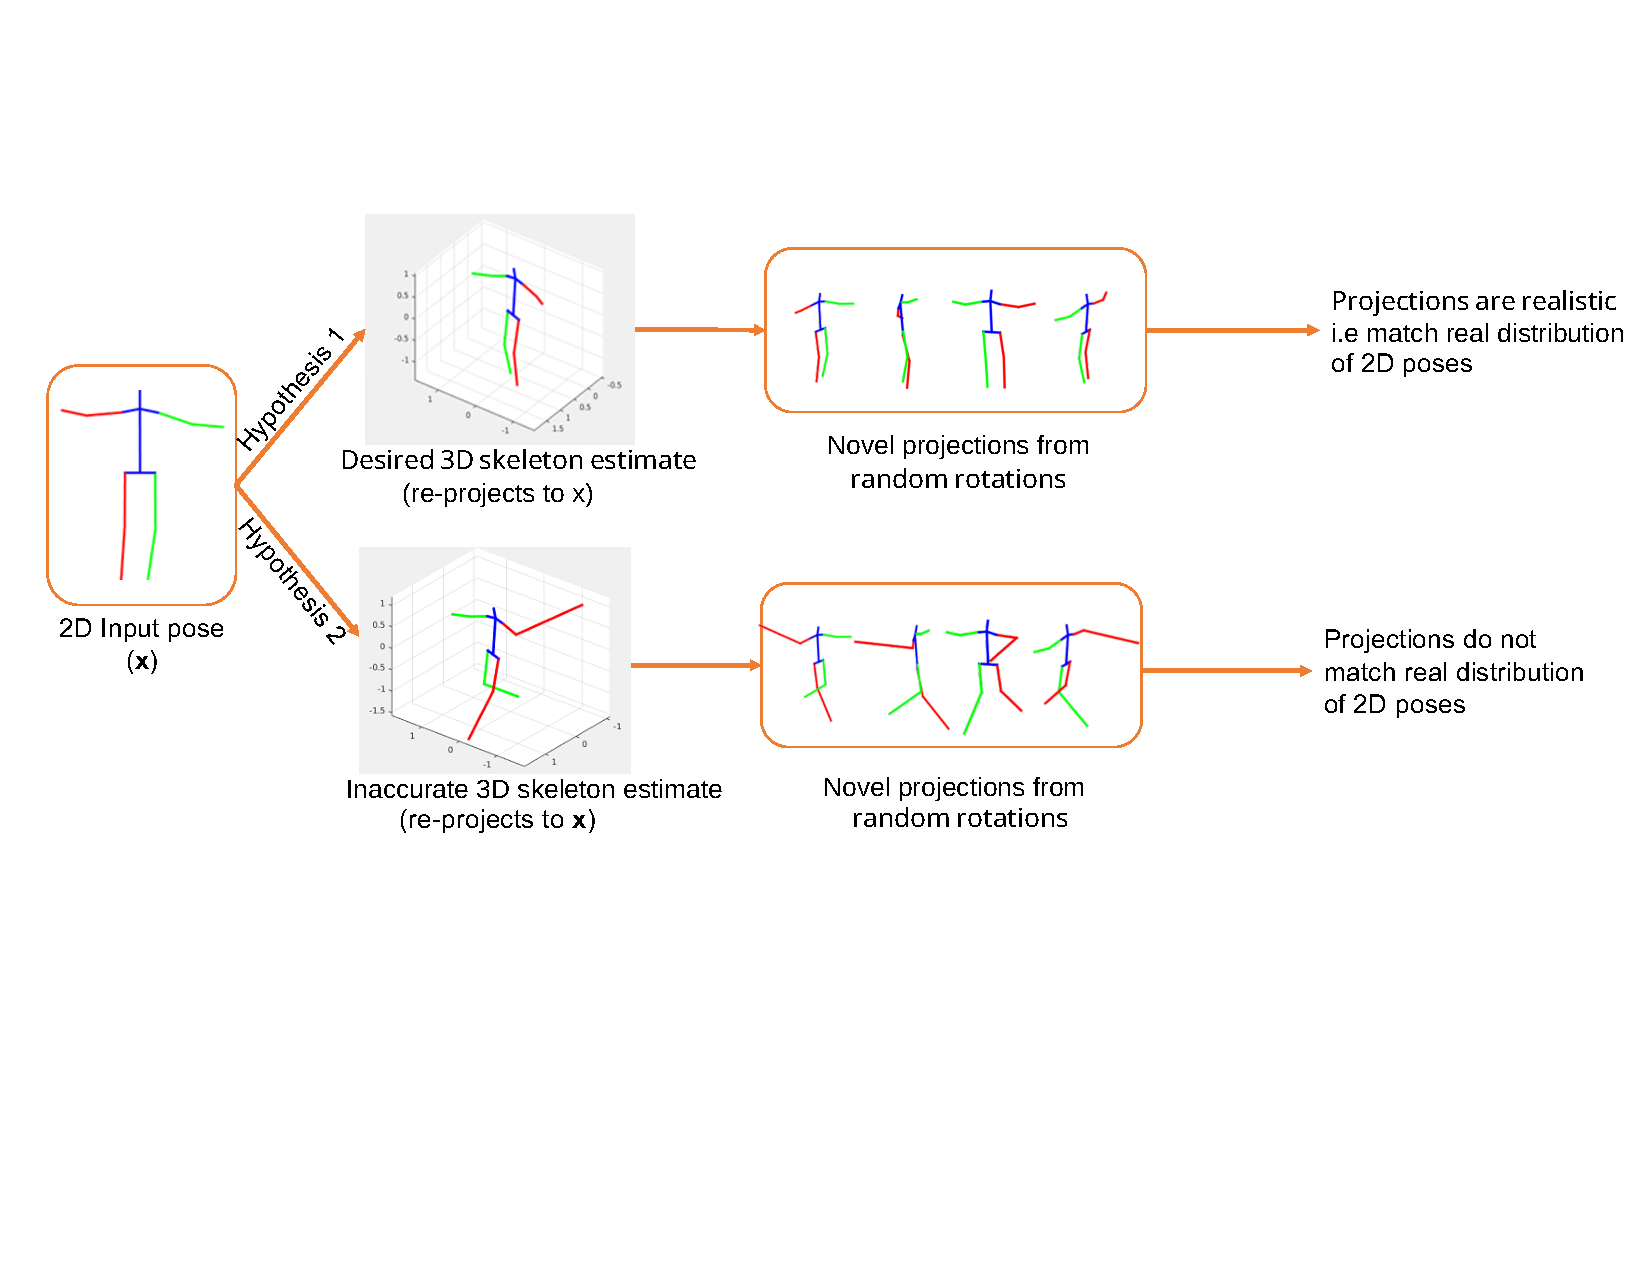
\includegraphics[width=\textwidth]{figures/h36_viz/novel_view_contraint.pdf}
    \caption{Illustration of the differences in accurate or realistic 3D pose predicitions from inaccurate predicitions. Modified image from \cite{can3dpose}}
    \label{fig:novel_view_constraint}
\end{figure}

The real and the fake 2D poses need not be related in any way. In practice, the loss terms of the real and fake data are computed and used to update the models separately, as suggested in \cite{soumith2017wasserstein, goodfellow2014generative}. As the goal of the discriminator is to just predict the correct label of the 2D pose, the \ac{bce} loss function is used. 

\begin{equation} \label{eqn:loss_bce}
    \begin{split}
        \mathcal{L}_{\text {Disc.}} & = BCE\_loss(y, \hat{y}) \\
        & = -1 * (\hat{y} \cdot \log y + (1 - \hat{y}) \cdot \log (1 - y)) \\
        & Where, \:\: y \in D_{\theta_d}(\tilde{\textbf{y}} \cup \textbf{x}) \;\; and \;\; \hat{y} \in (0s, 1s)
    \end{split}
\end{equation}

The $\tilde{\textbf{y}}$ here is the transformed output of the decoder. That means, to minimize this loss the decoder model is to be updated along with the discriminator. However, as discussed earlier we consider the encoder to be part of the generator. Hence all the models use this metric to update their weights. Again in contrast to the reconstruction loss, the discriminator loss does not give a direct signal to correct the 3D pose, and thus updating the models to minimize this loss is an unconstrained optimization and is not stable. Hence the weight coefficient $\lambda_{disc.}$ is not as high as that of the reconstruction loss. As this is a min-max game where the generator tries to fool the discriminator while the discriminator tries to guess which same is from the generator, all the models cannot be updated at the same time. The training procedure to enable the models to learn and improve the generated 3D pose is discussed in the next section.

\section{Training Procedure}

% \subsection{Procedure}
In this min-max game, the generator produces samples and the discriminator verifies them, the generator uses this verification and in our method, it also uses self-supervision loss to improve itself in both aspects. The standard practice in training \acp{gan} is to start with generating the samples using the generator. As the discriminator's evaluation is required to teach the generator, the discriminator is first trained to distinguish reals from fakes given by the generator. The samples are again given to the trained discriminator to get the loss to train the generator. That is, the generator is kept constant while updating the discriminator and the discriminator is kept constant while updating the generator. This turn-wise play is important without which the models would be trying to hit a moving target as put by \cite{gan_training_google}.

While the procedure seems straightforward, \ac{gan} training is finding a Nash equilibrium to a two-player non-cooperative game. There exists no feasible algorithm to find the equilibrium for a problem of such complexity\cite{improved_gan}. As the training initiates, the \ac{vae} produces 3D poses close to the noise and thus is very easy for the discriminator to learn to classify. This overpowers the discriminator as it predicts fakes with very high confidence and the loss tends to 0. The \ac{vae} can not learn properly if the discriminator does not provide proper feedback. This happens when the discriminator does not perform well or if it performs too well where the loss is close to 0 and not helpful \cite{gan_wgan_tutorial}. 

Other common challenges of \ac{gan} training and is explained in \ref{subsec:gan}. The widely practiced tricks to improve the training of \acp{gan} are discussed later in Bag of Tricks \ref{sec:bag_of_tricks}. The most challenging part of training any \acp{gan} is the lack of a proper metric to evaluate the quality of generations. Since it is difficult to monitor intermediate states in 3D, and since 3D poses have fewer features compared to RGB images, it is even more challenging to evaluate the quality of the generations. Hence more importance is given to the quantitative aspect in this report.

%TODO few details missing - more about problems of gans? how implemented? IDK IDC


\section{Evaluation} 

\subsection{Metric}
3D \ac{hpe} and Human3.6M in particular is evaluated by \ac{mpjpe} metric. \ac{mpjpe} as it abbreviates is the mean of the position estimate for all the joints of a pose. Where per-joint position estimate is nothing but the euclidian distance (measured in mm) between the predicted joint to its ground truth. The reported results refer to the average of the \ac{mpjpe} of all the samples in the evaluation set. 

\subsection{Protocols}
Human3.6M has 11 subjects out of which 7 are publically released while the rest are kept private. All the works main use of these 7 subjects for training and test. There are 2 widely used evaluation protocols. 

\paragraph{Protocol $\#1$} All the 4 camera views of subjects $S1$, $S5$, $S6$, $S7$, and $S8$ are used for training. Similarly, all camera views of subjects $S9$ and $S11$ are used for validation/testing. But the test subject data is complied by sampling every 64\textsuperscript{th} frame of the raw data while the train subjects data is made by sampling every 5\textsuperscript{th} frame. 
The evaluation metric \ac{mpjpe} calculation is done on the predicted 3D pose directly.

\paragraph{Protocol $\#2$} The train/test split is the same as of Protocol $\#1$. But \ac{mpjpe} is calculated on the predicted 3D after rigid body/ Procrustes alignment.

The design choice of predicting the 3D pose in unit scale makes it impossible to evaluate using protocol $\#1$. Hence, following \cite{amazon1}, results are reported using only protocol $\#2$ i.e after aligning the predicted 3D pose with the ground truth.

\subsection{Best Hypothesis}
During the evaluation phase, the discriminator network is discarded and the encoder and decoder pair alone is used. The usual practice during the evaluation phase of a \ac{vae} is to compute latent representation $z$ using mean and zeroing out the predicted standard deviation. The 3D pose prediction using the mean only is referred to $\textbf{ZV}$, Zero Variance. As the trained decoder can predict realistic 3D poses from any point in the latent space the variance can be scaled instead of zeroing to retrieve multiple 3D predictions for a 2D pose from which the mean is encoded. To evaluate the representation capability, 10 random hypotheses are produced following \cite{weaklymultiple}. This is done by randomly scaling the predicted variance vector. The best hypothesis, \textbf{BH} i.e the pose with the least \ac{mpjpe} for each 2D pose is selected to compute another variance of the mean \ac{mpjpe}. 
%TODOadd more
